%%%%%%%%%%%%%%%%%%%%%%%%%%%%%%%%%%%%%%%%%
% Short Sectioned Assignment LaTeX Template Version 1.0 (5/5/12)
% This template has been downloaded from: http://www.LaTeXTemplates.com
% Original author:  Frits Wenneker (http://www.howtotex.com)
% License: CC BY-NC-SA 3.0 (http://creativecommons.org/licenses/by-nc-sa/3.0/)
%%%%%%%%%%%%%%%%%%%%%%%%%%%%%%%%%%%%%%%%%

%----------------------------------------------------------------------------------------
%	PACKAGES AND OTHER DOCUMENT CONFIGURATIONS
%----------------------------------------------------------------------------------------

\documentclass[paper=a4, fontsize=11pt]{scrartcl} % A4 paper and 11pt font size

% ---- Entrada y salida de texto -----

\usepackage[T1]{fontenc} % Use 8-bit encoding that has 256 glyphs
\usepackage[utf8]{inputenc}
%\usepackage{fourier} % Use the Adobe Utopia font for the document - comment this line to return to the LaTeX default

% ---- Idioma --------

\usepackage[spanish, es-tabla]{babel} % Selecciona el español para palabras introducidas automáticamente, p.ej. "septiembre" en la fecha y especifica que se use la palabra Tabla en vez de Cuadro

% ---- Otros paquetes ----

\usepackage{url} % ,href} %para incluir URLs e hipervínculos dentro del texto (aunque hay que instalar href)
\usepackage{amsmath,amsfonts,amsthm} % Math packages
%\usepackage{graphics,graphicx, floatrow} %para incluir imágenes y notas en las imágenes
\usepackage{graphics,graphicx, float} %para incluir imágenes y colocarlas

% Para hacer tablas comlejas
%\usepackage{multirow}
%\usepackage{threeparttable}

%\usepackage{sectsty} % Allows customizing section commands
%\allsectionsfont{\centering \normalfont\scshape} % Make all sections centered, the default font and small caps

\usepackage{fancyhdr} % Custom headers and footers
\pagestyle{fancyplain} % Makes all pages in the document conform to the custom headers and footers
\fancyhead{} % No page header - if you want one, create it in the same way as the footers below
\fancyfoot[L]{} % Empty left footer
\fancyfoot[C]{} % Empty center footer
\fancyfoot[R]{\thepage} % Page numbering for right footer
\renewcommand{\headrulewidth}{0pt} % Remove header underlines
\renewcommand{\footrulewidth}{0pt} % Remove footer underlines
\setlength{\headheight}{13.6pt} % Customize the height of the header

\numberwithin{equation}{section} % Number equations within sections (i.e. 1.1, 1.2, 2.1, 2.2 instead of 1, 2, 3, 4)
\numberwithin{figure}{section} % Number figures within sections (i.e. 1.1, 1.2, 2.1, 2.2 instead of 1, 2, 3, 4)
\numberwithin{table}{section} % Number tables within sections (i.e. 1.1, 1.2, 2.1, 2.2 instead of 1, 2, 3, 4)

\setlength\parindent{0pt} % Removes all indentation from paragraphs - comment this line for an assignment with lots of text

\newcommand{\horrule}[1]{\rule{\linewidth}{#1}} % Create horizontal rule command with 1 argument of height

%\documentclass{report}
\usepackage{blindtext}
\usepackage{hyperref}
\usepackage{listings}
\usepackage{graphicx}
\graphicspath{ {images/} }

\title{	
\normalfont \normalsize 
\textsc{\textbf{Ingeniería de Servidores (2022-2023)} \\ Grado en Ingeniería Informática \\ Universidad de Granada} \\ [25pt] % Your university, school and/or department name(s)
\horrule{0.5pt} \\[0.4cm] % Thin top horizontal rule
\huge Memoria Práctica 3 \\ % The assignment title
\horrule{2pt} \\[0.5cm] % Thick bottom horizontal rule
}

\author{Francisco Javier Gallardo Molina} % Nombre y apellidos

\date{\normalsize\today} % Incluye la fecha actual

\renewcommand{\footrulewidth}{0.4pt}
\lfoot[]{Francisco Javier Gallardo Molina}
\rfoot[]{\thepage}

\begin{document}

\maketitle

\newpage

\horrule{1pt}
\tableofcontents

\newpage

\section{Instalación de máquinas virtuales}

Para la realización de esta práctica, debemos de hacer una instalación de dos máquinas virtuales, una que haga de servidor y una de cliente. Para la máquina servidor se usará Ubuntu 20.04 y para el cliente Rocky Linux 9.0. Para cada máquina debemos tener un sistema de archivos RAID1 instalado, por lo que debemos tener la siguiente configuración en Ubuntu como se ve en la figura \ref{fig:lsblk-ubuntu}.

\begin{figure}[H]
  \centering
  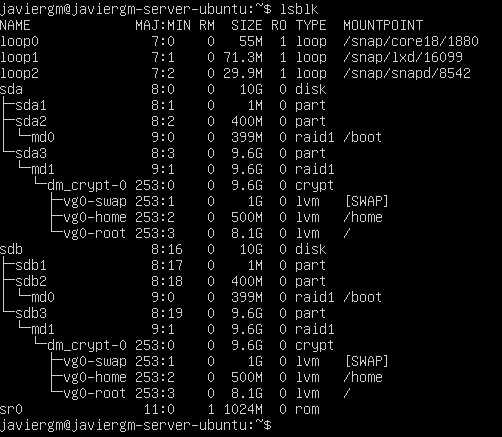
\includegraphics[scale=0.9]{Captura1}
  \caption{Sistema de archivos RAID1 en Ubuntu}
  \label{fig:lsblk-ubuntu}
\end{figure}

De igual manera, Rocky debe de tener una configuración similar a esta figura \ref{fig:lsblk-rocky}.\\

\begin{figure}[H]
  \centering
  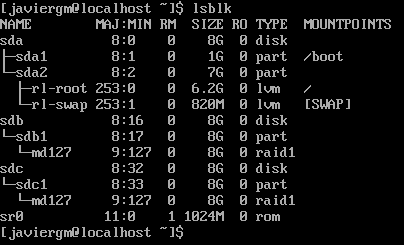
\includegraphics[scale=0.9]{Captura2}
  \caption{Sistema de archivos RAID1 en Rocky Linux}
  \label{fig:lsblk-rocky}
\end{figure}

\section{Zabbix}

\subsection{Instalación y configuración del servidor en Ubuntu 20}
Para la instalación de Zabbix en la máquina virtual he seguido este manual 
\url{https://www.zabbix.com/download?zabbix=5.0&os_distribution=ubuntu&os_version=20.04_focal&db=mysql&ws=apache} para instalar el servidor y el agente de Zabbix.\\

Lo primero que hay que hacer es instalar el repositorio de Zabbix en la máquina usando los siguientes comandos:

\begin{lstlisting}
> wget  https://repo.zabbix.com/zabbix/5.0/ubuntu/pool/main/z/
zabbix-release/zabbix-release_5.0-1+focal_all.deb
\end{lstlisting}

\begin{lstlisting}
> sudo dpkg -i zabbix-release_5.0-1+focal_all.deb
\end{lstlisting}

\begin{lstlisting}
> sudo apt update
\end{lstlisting}

Tras instalar el repositorio, en lugar de usar un proxy para la instalación he preferido seguir con este manual \url{https://www.zabbix.com/download?zabbix=5.0&os_distribution=debian&os_version=10_buster&db=mysql} y usar los paquetes de zabbix de frontend, servidor y agente:

\begin{lstlisting}
> sudo apt install zabbix-server-mysql zabbix-frontend-php 
zabbix-apache-conf zabbix-agent 
\end{lstlisting}

Con todo ya instalado, procedemos a configurar la base de datos con la que Zabbix va a trabajar. Para ello, primero tenemos que instalar la base de datos, que en mi caso será MySQL:

\begin{lstlisting}
> sudo apt install mysql-server
\end{lstlisting}

Una vez instalada, debemos crear la base de datos que el servidor usará. Para ello debemos de entrar en el prompt de MySQL con el siguiente comando:

\begin{lstlisting}
> sudo mysql -u root -p
\end{lstlisting}

Cabe destacar que tras ejecutar este comando nos pedirá contraseña, pero al no haber hecho una configuración previa, no habrá que introducir nada y nos permitirá entrar en el prompt de la base de datos sin problemas. Dentro de este prompt, realizamos la configuración que se indica en la documentación de Zabbix o en la figura \ref{fig:mysql}.

\begin{figure}[H]
  \centering
  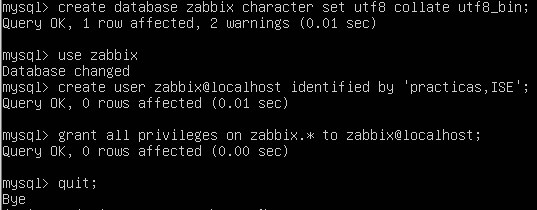
\includegraphics{Captura3}
  \caption{Configuración de la base de datos de Zabbix}
  \label{fig:mysql}
\end{figure}

Una vez creada la base de datos, seguimos la documentación de Zabbix y ejecutamos el siguiente comando:\\

\begin{lstlisting}
> zcat /usr/share/doc/zabbix-server-mysql*/create.sql.gz | mysql
-uzabbix -p zabbix
\end{lstlisting}

Nos pedirá una contraseña y debemos de meter la que se ha indicado en la \ref{fig:mysql}, que en mi caso es \textit{practicas,ISE}. Después de esto, saltó un error de los discos bastante grande \ref{fig:error}.

\begin{figure}[H]
  \centering
  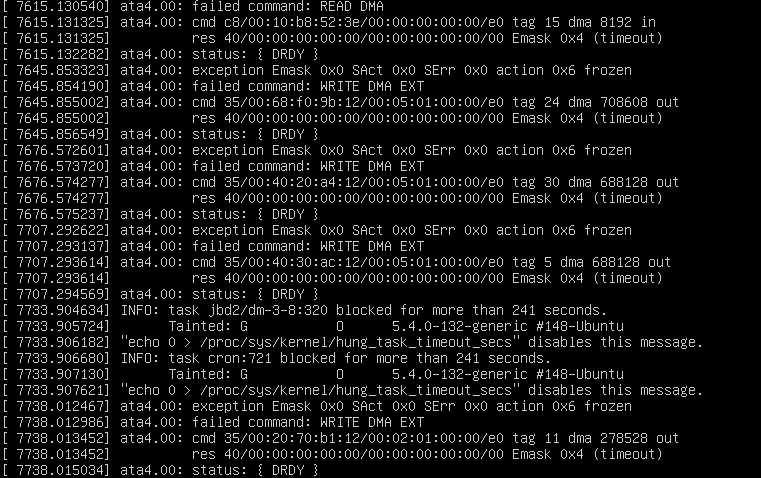
\includegraphics[scale=0.9]{error}
  \caption{Error mostrado}
  \label{fig:error}
\end{figure}

Puesto que no me dejó realizar ninguna acción, tuve que matar el proceso de VirtualBox para poder apagar la máquina. Tras eso, encendí de nuevo la máquina esperando que se hubiera roto todo, pero sorprendentemente, no hubo problemas al iniciar. Probé a introducir el comando de nuevo, pero me mostró por pantalla que los datos estaban ya creados, así que aparentemente todo estaba normal,  por lo que decidí continuar con la instalación.\\

Con todo esto hecho, pasamos a modificar los archivos de configuración de Zabbix para indicarle cuál es la contraseña que hemos introducido. Para ello nos vamos al archivo '/etc/zabbix/zabbix\_server.conf' y modificamos la sección en la que pone 'DBPassword', descomentamos la instrucción y ponemos nuestra contraseña como se indica en la figura \ref{fig:zabbix-conf}.

\begin{figure}[H]
  \centering
  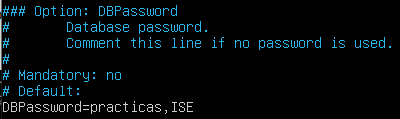
\includegraphics{Captura4}
  \caption{Contraseña de Zabbix en archivo de configuración}
  \label{fig:zabbix-conf}
\end{figure}

Por último modificamos el archivo '/etc/zabbix/apache.conf' para cambiar el huso horario de nuestro servidor de Zabbix como se indica la figura \ref{fig:zabbix-conf-apache}:

\begin{figure}[H]
  \centering
  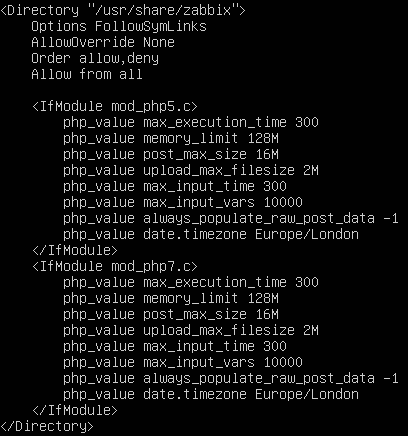
\includegraphics[scale=0.9]{Captura5}
  \caption{Huso horario de Zabbix}
  \label{fig:zabbix-conf-apache}
\end{figure}

Con todo esto hecho, reiniciamos el servidor de Zabbix junto con su agente y apache2:

\begin{lstlisting}
> sudo systemctl restart zabbix-server zabbix-agent apache2
\end{lstlisting}

\begin{lstlisting}
> sudo systemctl enable zabbix-server zabbix-agent apache2 
\end{lstlisting}

Tras esto, comprobamos que los servicios de MySQL, Apache2 y Zabbix estén funcionando, como aparece en las figuras \ref{fig:estado-mysql}, \ref{fig:estado-apache} y \ref{fig:estado-zabbix}.


\begin{figure}[H]
  \centering
  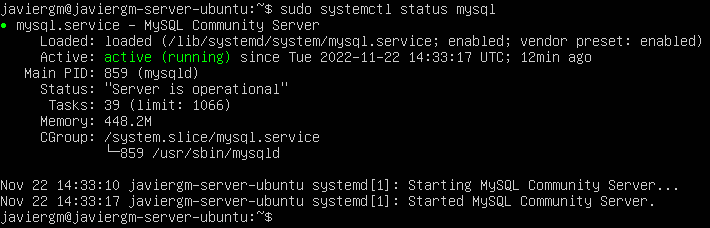
\includegraphics[scale=0.9]{Captura6}
  \caption{Estado del servicio de MySQL}
  \label{fig:estado-mysql}
\end{figure}

\begin{figure}[H]
  \centering
  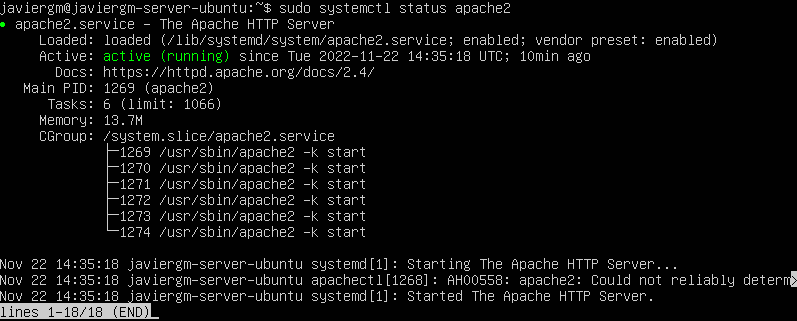
\includegraphics[scale=0.9]{Captura7}
  \caption{Estado del servicio de Apache2}
  \label{fig:estado-apache}
\end{figure}

\begin{figure}[H]
  \centering
  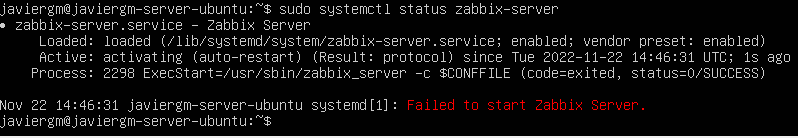
\includegraphics[scale=0.9]{Captura8}
  \caption{Estado del servicio de Zabbix-server}
  \label{fig:estado-zabbix}
\end{figure}

Al comprobar el estado de Zabbix, vemos que ha fallado al iniciar el servicio. Este error tras investigar junto con la ayuda del profesor, vimos que se debía a un fallo al importar los datos a la base de datos y que está relacionado con el error \ref{fig:error}. Para solucionarlo, tuvimos que borrar la base de datos de Zabbix y volverla a crear, pero al tratar de crear los datos del usuario de Zabbix, nos mostraba por pantalla que no se podía. Al final la solución fue realizar esta serie de comandos:

\begin{lstlisting}
mysql> drop user zabbix@localhost; 
\end{lstlisting}

\begin{lstlisting}
mysql> flush privileges;
\end{lstlisting}

\begin{lstlisting}
mysql> create user zabbix@localhost identified by 'practicas,ISE'
\end{lstlisting}

\begin{lstlisting}
mysql> grant all privileges on zabbix.* to zabbix@localhost;
\end{lstlisting}

Una vez hecho esto, volvimos a importar los datos de Zabbix con el comando:

\begin{lstlisting}
> zcat /usr/share/doc/zabbix-server-mysql*/create.sql.gz | mysql
-uzabbix -p zabbix
\end{lstlisting}

Nos volvió a pedir la contraseña, y tras introducirla, se copiaron los datos sin que saltara el error \ref{fig:error}. Puesto que parece estar todo correcto, probamos a comprobar el estado del servicio de Zabbix-server \ref{fig:estado-zabbix-correcto}.

\begin{figure}[H]
  \centering
  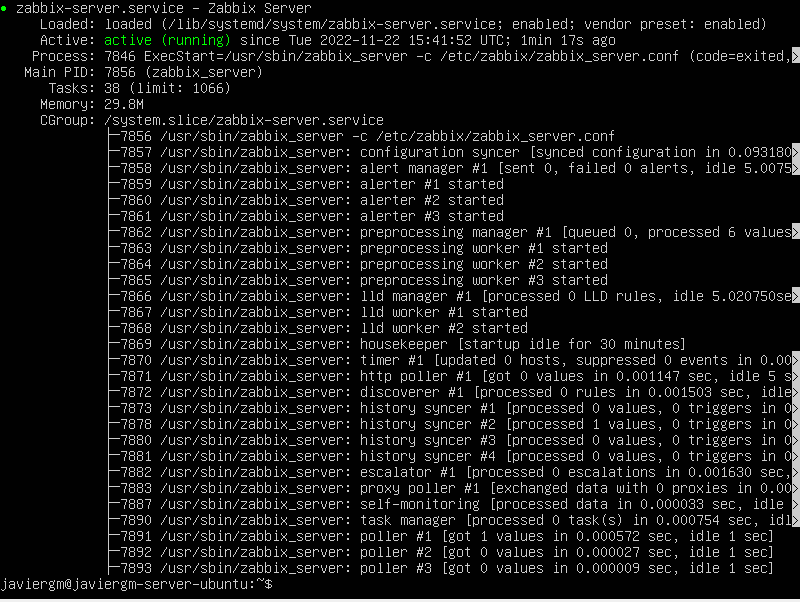
\includegraphics[scale=0.7]{Captura9}
  \caption{Estado del servicio de Zabbix-server}
  \label{fig:estado-zabbix-correcto}
\end{figure}

Puesto que ya funciona, la configuración del servidor está terminada.\\

Como parte opcional, para hacer la instalación de la base de datos de MySQL más segura, es recomendable usar el comando de "mysql\_secure\_installation" para ajustar ciertos parámetros como establecer una contraseña para la cuenta de root o desactivar el acceso remoto al usuario root.\\

Si bien con todo esto ya podríamos usar el servidor de Zabbix para monitorizar el servidor puede ser que no podamos acceder a Zabbix desde el navegador, como ocurrió en mi caso. Puede ser debido a que la interfaz de red no tenga asignada una IP con la que se pueda conectar a la máquina virtual o que no tenga el adaptador de red solo-anfitrión activado. Para que funcione, debemos de activar otro adaptador de red en VirtualBox que sea solo-anfitrión como indica la figura \ref{fig:adaptador}.\\

\begin{figure}[H]
  \centering
  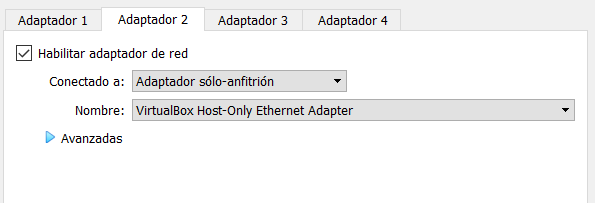
\includegraphics{Captura10}
  \caption{Adaptador solo-anfitrión}
  \label{fig:adaptador}
\end{figure}

Tras esto, ejecutamos 'ip addr' para comprobar su dirección IP, pero vemos que no aparece nada. Debemos de asociarle una IP y activar la interfaz con los siguientes comandos:

\begin{lstlisting}
> sudo ip addr add 192.168.56.115/24 dev enp0s8
\end{lstlisting}

\begin{lstlisting}
> sudo ip link set enp0s8 up
\end{lstlisting}

\begin{figure}[H]
  \centering
  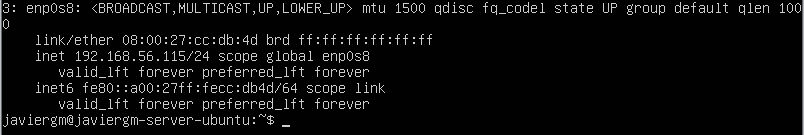
\includegraphics[scale=0.8]{Captura11}
  \caption{IP de la máquina}
  \label{fig:ip}
\end{figure}

Un problema que puede surgir es que el cortafuegos de Windows, como es mi caso, no nos permita conectarnos a Zabbix desde el navegador. Debemos de entrar en la configuración avanzada del cortafuegos y en el apartado de \textit{Reglas de entrada} añadimos una regla que permita la conexión de nuestro PC con la máquina virtual a través de las IPs.\\

Realizado todo el proceso de la IP, ya podemos proceder a instalar y configurar el frontend de Zabbix. Es un proceso rápido por lo que no tiene mucha complicación. Debemos de indicar la base de datos de Zabbix y su contraseña \ref{fig:conf-frontend}. El resto de configuración lo dejamos por defecto.

\begin{figure}[H]
  \centering
  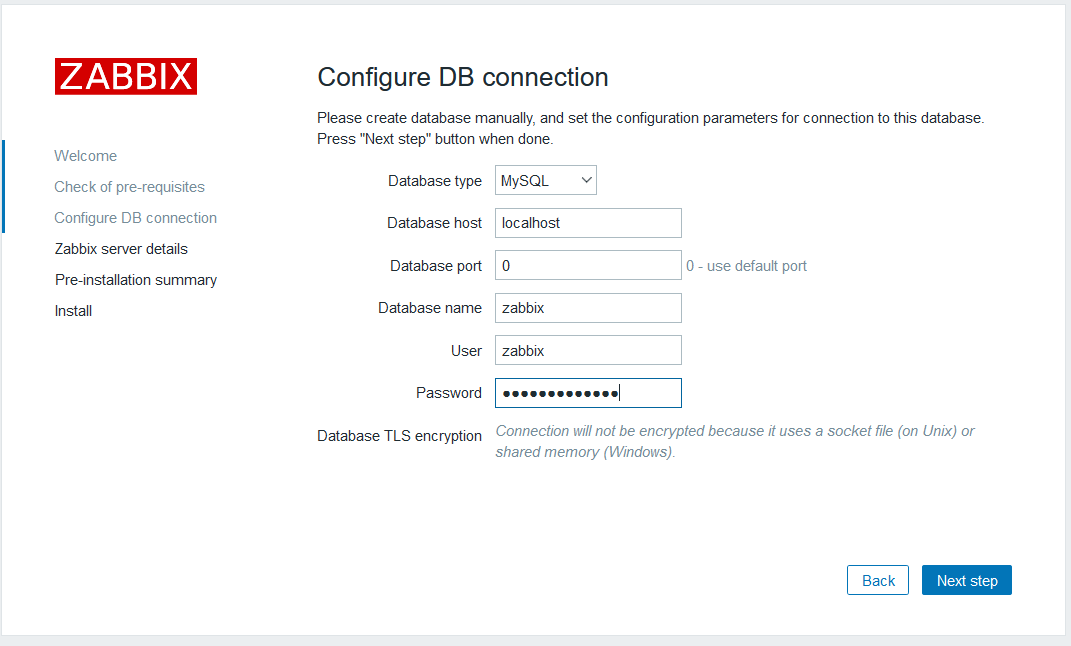
\includegraphics[scale=0.6]{Captura12}
  \caption{Configuración de Zabbix en navegador}
  \label{fig:conf-frontend}
\end{figure}

Por úlitmo, nos pedirá que iniciemos sesión y usaremos el usuario por defecto \textit{Admin} y la contraseña \textit{zabbix}. Iniciando sesión, ya tendremos listo nuestro servidor para monitorizar.\\

Cabe destacar que para que Ubuntu se monitorice a sí mismo debe de usar el agente de Zabbix e indicar en su configuración la dirección IP del servidor para que funcione correctamente, si no, en la página del navegador de Zabbix mostrará un fallo cuando se trate de monitorizar Ubuntu.

\newpage
\subsection{Instalación del agente en Rocky Linux 9}

Para la instalación del agente en Rocky he seguido este manual 
\url{https://www.zabbix.com/download?zabbix=5.0&os_distribution=rocky_linux&os_version=9&components=agent&db=&ws=}.

Usamos los siguientes comandos para obtener el repositorio:

\begin{lstlisting}
# rpm -Uvh https://repo.zabbix.com/zabbix/5.0/rhel/
8/x86_64/zabbix-release-5.0-1.el8.noarch.rpm
# dnf clean all 
\end{lstlisting}

Habiendo añadido el repositorio, procedemos a instalar el agente de Rocky:

\begin{lstlisting}
# sudo dnf install zabbix-agent
\end{lstlisting}

Tras esto iniciamos el servicio de Zabbix:

\begin{lstlisting}
# systemctl restart zabbix-agent
# systemctl enable zabbix-agent
\end{lstlisting}

Para configurar el agente de Zabbix, debemos de activar el adaptador solo-anfitrión de la máquina de Rocky y asignarle una dirección IP como hicimos anteriormente con Ubuntu \ref{fig:adaptador}. Para Rocky le asignamos la IP \textit{192.168.56.110/24}. 

Tras esto, procedemos a configurarlo en su archivo \textit{/etc/zabbix/zabbix\_agentd.conf} para añadir la IP del servidor y la IP donde tiene que escuchar el agente (la IP de la propia máquina de Rocky)\ref{fig:agent}.

\begin{figure}[H]
  \centering
  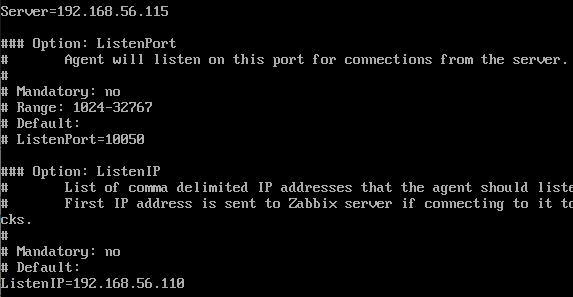
\includegraphics[scale=0.7]{Captura13}
  \caption{Configuración de Zabbix-agent en Rocky}
  \label{fig:agent}
\end{figure}

Como indica la figura, la IP que aparece primero es la del servidor de Zabbix en Ubuntu y en la última línera de la captura aparece la IP de Rocky. Es importante que la máquina tenga una IP asociada, pues si no, la configuración del agente fallará y el servicio de Zabbix-agent no se iniciará.\\

El cortafuegos de Rocky es una parte importante de la configuración, pues debemos de añadir una regla para que permita el tráfico de paquetes en el puerto 10050. Para ellos ejecutamos los siguientes comandos:

\begin{lstlisting}
# sudo firewall-cmd --add-port=10050/tcp --permanent
# sudo firewall-cmd --reload
\end{lstlisting}

De esta forma añadimos de forma permanente la regla y hacemos que el cortafuegos permita el tráfico por el puerto 10050. 

\newpage
\subsection{Monitorización de las máquinas}

Ahora pasaremos al navegador y entramos en la Dashboard de Zabbix para empezar a monitorizar las dos máquinas virtuales.\\

Lo primero que debemos hacer es crear los hosts para que Zabbix pueda monitorizar las máquinas. Nos vamos al apartado de \textit{Configuration > Hosts} y le damos al botón de \textit{Create host}. Rellenamos los datos necesarios, indicando la IP a la que se tiene que conectar \ref{fig:host-config}.

\begin{figure}[H]
  \centering
  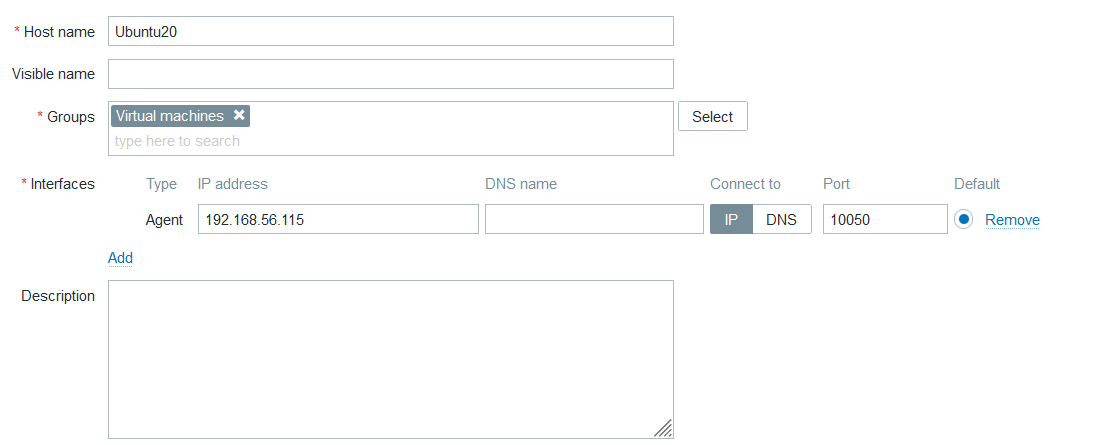
\includegraphics[scale=0.7]{Captura14}
  \caption{Configuración de los hosts en Zabbix}
  \label{fig:host-config}
\end{figure}

Hacemos lo mismo para Rocky, de tal forma que tendremos los dos hosts creados más el host por defecto \ref{fig:host-creados}.

\begin{figure}[H]
  \centering
  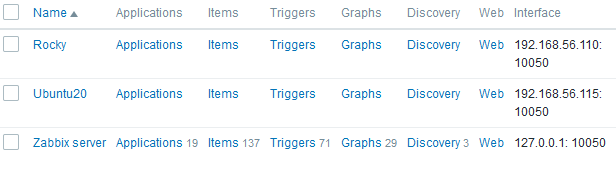
\includegraphics[scale=0.8]{Captura15}
  \caption{Hosts creados}
  \label{fig:host-creados}
\end{figure}

Para cada host, clicamos en el apartado de items para indicar qué datos tiene que analizar Zabbix de las máquinas y le damos al botón de \textit{Create item}. Para Ubuntu y para Rocky realizamos el mismo paso \ref{fig:items-creados}:

\begin{figure}[H]
  \centering
  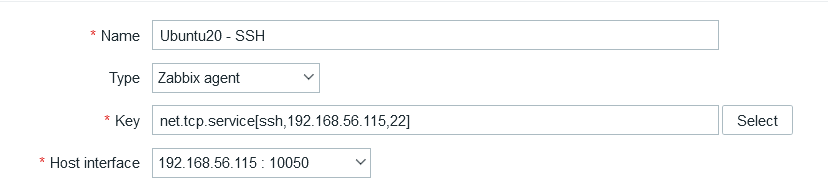
\includegraphics[scale=0.9]{Captura16}
  \caption{Items de monitorización creados}
  \label{fig:items-creados}
\end{figure}

Esta opción es para crear un item personal con parámetros que nosotros queramos especificar (en este caso sobre SSH), pero existen templates que vienen por defecto para monitorizar ciertos aspectos de las máquinas. En nuestro caso, tenemos que monitorizar los servicios SSH, HTTP y el uso de la CPU, la memoria, etcétera, pero podemos añadir más servicios para monitorizar. Usaremos los templates por defecto para poder ver HTTP y otros servicios(entre ellos la monitorización de los discos) \ref{fig:templates}:

\begin{figure}[H]
  \centering
  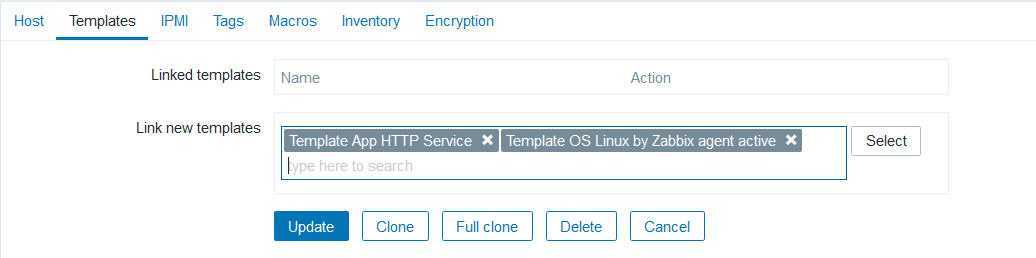
\includegraphics[scale=0.6]{Captura17}
  \caption{Templates de monitorización}
  \label{fig:templates}
\end{figure}

Añadiendo estos templates tanto en Ubuntu como en Rocky ya podemos ver cuando los servicios están funcionando o no. Podemos probar a parar el servidor de SSH de Ubuntu y volverlo a encender para comprobar que en Zabbix podemos ver cuando está activo y cuando no en \textit{Monitoring > Latest data} \ref{fig:monit-servicios}:

\begin{figure}[H]
  \centering
  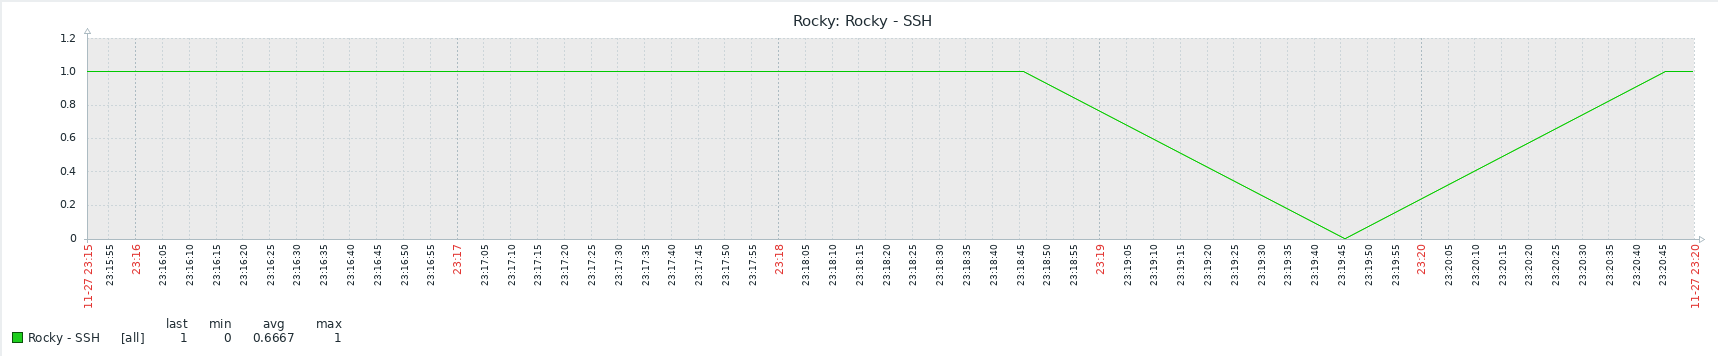
\includegraphics[scale=0.4]{Captura18}
  \caption{Monitorización de los servicios}
  \label{fig:monit-servicios}
\end{figure}

En este ejemplo podemos ver que el servicio de SSH que hemos parado voluntariamente durante un periodo corto de tiempo para luego ponerlo a funcionar lo ha captado Zabbix.

\newpage

\section{Ansible}

\subsection{Instalación}
Para la instalación de Ansible, he instalado otra máquina virtual con Rocky Linux. He seguido esta documentación \url{https://docs.rockylinux.org/books/learning_ansible/01-basic/}. Aquí nos pone dos maneras de instalar Ansible, usando EPEL o usando Python. En mi caso lo instalaré a través de EPEL. Para ello usaré estos comandos:

\begin{lstlisting}
# sudo dnf install epel-release
\end{lstlisting}

\begin{lstlisting}
# sudo dnf install ansible
\end{lstlisting}

Una vez hecho esto podemos comprobar la versión de Ansible para comprobar cuál tenemos \ref{fig:ansible-version}.

\begin{figure}[H]
  \centering
  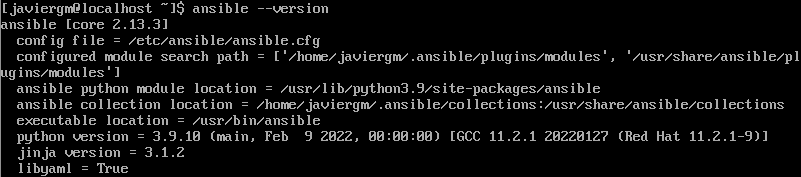
\includegraphics[scale=0.8]{Captura19}
  \caption{Versión de Ansible}
  \label{fig:ansible-version}
\end{figure}

Por el funcionamiento de Ansible, debemos de tener instalado OpenSSH para poder ejecutar comandos ya que manda las peticiones a través SSH. 

\newpage
\subsection{Configuración y uso}

Para que ansible se ejecute, debemos de especificar en el archivo "hosts" de la ruta "/etc/ansible/" todas las IPs donde queremos ejecutar Ansible. Puesto que nosotros solamente queremos ejecutar un par de comandos en nuestro servidor de Ubuntu y de Rocky (donde tenemos el zabbix-agent), añadimos las IPs de las dos máquinas a nuestra máquina cliente. También podemos añadir el nombre de dominio donde queramos ejecutar los comandos. Solamente debemos de añadir la url. Puesto que este no es nuestro caso, solo nos basta con poner la IP. Si en el momento en el que instalamos openssh en nuestro servidor cambiamos el puerto de acceso, debemos de indicar en la IP el puerto también \ref{fig:ansible-hosts}.

\begin{figure}[H]
  \centering
  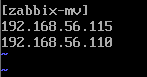
\includegraphics{Captura20}
  \caption{Hosts de Ansible}
  \label{fig:ansible-hosts}
\end{figure}

Ya podemos probar a ejecutar el siguiente comando:

\begin{lstlisting}
# ansible zabbix-mv -m ping
\end{lstlisting}

Tras ejecutarlo obtenemos el siguiente resultado \ref{fig:ansible-prueba}.

\begin{figure}[H]
  \centering
  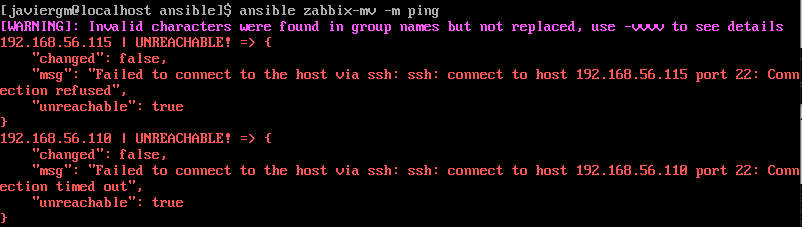
\includegraphics[scale=0.8]{Captura21}
  \caption{Resultado del comando de Ansible}
  \label{fig:ansible-prueba}
\end{figure}

Puede ser que falle el comando, pues nos pide autenticación, como nos indica la documentación. Una de las soluciones es usar claves rsa e intercambiarlas para no tener que autenticarnos por contraseña. Para ello hacemos uso de estos comandos: 

\begin{lstlisting}
# ssh-keygen -t rsa -b 4096
\end{lstlisting}

\begin{lstlisting}
# ssh-copy-id 192.168.56.115
\end{lstlisting}

Cabe destacar que en Rocky no funcionará de primeras, por lo que primero debemos de permitir en el cortafuegos que pasen los paquetes en el puerto que tengamos en SSH, por lo que para que funcione también en Rocky, debemos usar estos comandos:

\begin{lstlisting}
# sudo firewall-cmd --add-port=22/tcp --permanent
\end{lstlisting}

\begin{lstlisting}
# sudo firewall-cmd --reload
\end{lstlisting}

\begin{lstlisting}
# ssh-copy-id 192.168.56.110
\end{lstlisting}

Tras hacer esto, ya sí debería funcionar todo. Haciendo de nuevo la prueba de Ansible tenemos el siguiente resultado \ref{fig:ansible-prueba-2}:

\begin{figure}[H]
  \centering
  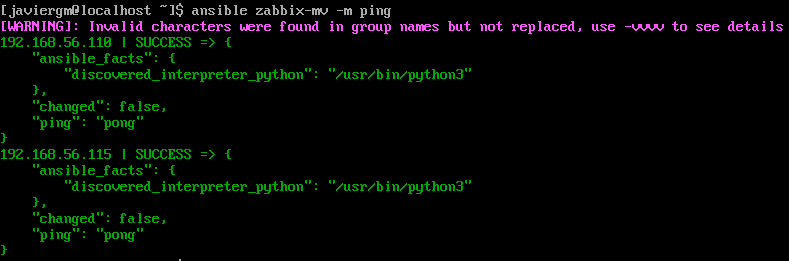
\includegraphics[scale=0.8]{Captura22}
  \caption{Resultado del comando de Ansible}
  \label{fig:ansible-prueba-2}
\end{figure}

En la imagen se puede ver que ya funciona de forma correcta hacer un ping a las máquinas, así que ahora ya se puede probar realizar un comando básico como por ejemplo el script de monitorización del sistema de RAID1. Para ello usamos el siguiente comando: 

\begin{lstlisting}
# ansible zabbix-mv -m shell -a "cat /proc/mdstat"
\end{lstlisting}

Usando este comando en mi máquina de Rocky obtengo el siguiente resultado \ref{fig:ansible-mdstat}:

\begin{figure}[H]
  \centering
  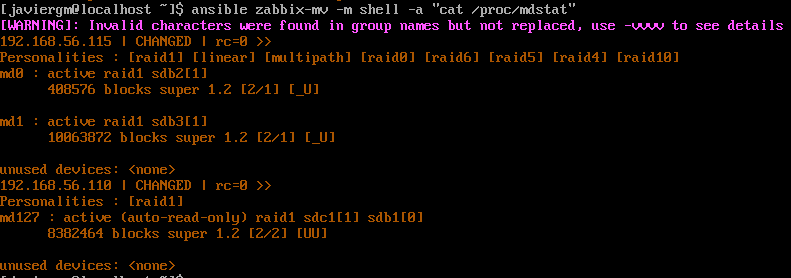
\includegraphics[scale=0.8]{Captura23}
  \caption{Resultado del comando de Ansible}
  \label{fig:ansible-mdstat}
\end{figure}

Vemos que el comando se ejecuta correctamente y nos muestra el resultado del script, que de hecho, ejecutando este comando me di cuenta de que uno de los dos discos del RAID1 de la máquina de Ubuntu no funciona. Haciendo una retrospectiva a todo lo realizado, ese disco seguramente dejó de funcionar en el momento en el que saltó este error \ref{fig:error}. Para arreglar este problema hay que añadir otro disco a la máquina y añadirlo al RAID1 usando el comando de mdadm.

\newpage
\subsection{Uso de playbooks}

Si bien lo mostrado anteriormente funciona, también podemos usar playbooks para realizar la ejecución como si fuera un script y realizar acciones más complejas. Debemos de crear un archivo "playbook.yml". En él debemos de escribir las instrucciones que queremos que realice \ref{fig:ansible-playbook}.

\begin{figure}[H]
  \centering
  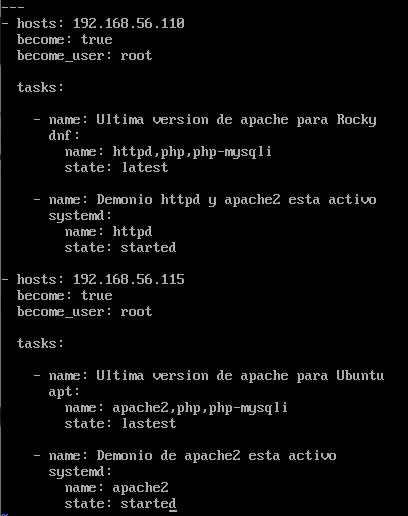
\includegraphics[scale=0.8]{Captura24}
  \caption{Playbook de Ansible}
  \label{fig:ansible-playbook}
\end{figure}

En este playbook he indicado que en el grupo de hosts las IPs de cada máquina se ejecute como root y compruebe si los demonios del servidor apache están en funcionamiento y si su versión es la última. Cuando tengamos el playbook listo, debemos ejecutarlo de la siguente forma:

\begin{lstlisting}
# ansible-playbook playbook.yml
\end{lstlisting}

Tras ejecutarlo vemos el resultado \ref{fig:ansible-playbook-res}: 

\begin{figure}[H]
  \centering
  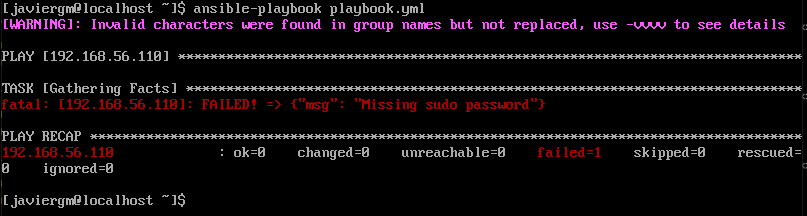
\includegraphics[scale=0.8]{Captura25}
  \caption{Resultado del playbook}
  \label{fig:ansible-playbook-res}
\end{figure}


En la imagen podemos comprobar que no tenemos permisos para ejecutar como root, por lo que debemos de darle permisos a Ansible como indica la documentación.\\

Primero de todo nos logueamos como superusuario con el comando de \textit{sudo su} para poder modificar el archivo de \textit{/etc/ansible/ansible.cfg} y cambiar el campo de \textit{aks\_pass} a True en nuestra máquina donde ejecutamos Ansible. A continuación debemos de realizar en la máquina de Rocky con el zabbix-agent los siguientes comandos:

\begin{lstlisting}
# sudo useradd ansible
\end{lstlisting}

\begin{lstlisting}
# sudo usermod -aG wheel ansible
\end{lstlisting}

Con esto añadimos el usuario de Ansible a la rueda de wheel de permisos de root. A continuación añadimos contraseña al usuario:

\begin{lstlisting}
# sudo passwd ansible
\end{lstlisting}

Después de esto, en el archivo de \textit{visudo} cambiamos que todos los usuarios de wheel puedan ejecutar todos los comandos sin que nos pida contraseña con este comando:

\begin{lstlisting}
# sudo visudo
\end{lstlisting}

Debemos modificar los campos y que se queden como se indica aquí abajo:

\begin{lstlisting}
## Allows people in group wheel to run all commands
# %wheel  ALL=(ALL)       ALL

## Same thing without a password
%wheel        ALL=(ALL)       NOPASSWD: ALL
\end{lstlisting}

Con esto ya podemos ejecutar el playbook  con Rocky solamente. Si lo hacemos de nuevo, obtenemos lo siguiente \ref{fig:ansible-playbook-wheel}:

\begin{figure}[H]
  \centering
  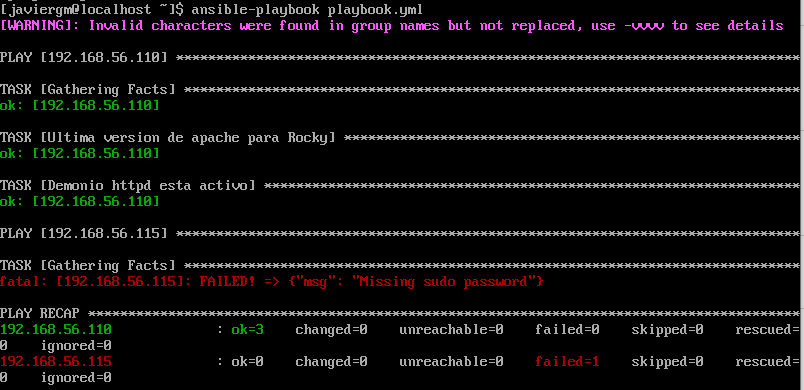
\includegraphics[scale=0.6]{Captura26}
  \caption{Playbook de Ansible}
  \label{fig:ansible-playbook-wheel}
\end{figure}

Con esta ejecución podemos ver que el playbook se puede ejecutar en Rocky, pero no en Ubuntu, y que además se comprueba que el servicio de httpd está activo y está en su última versión. Ahora debemos de darle permisos a Ubuntu para que realice la misma tarea. Para ello, creamos el usuario de Ansible en Ubuntu y lo añadimos al grupo de sudoers:

\begin{lstlisting}
# sudo useradd ansible
\end{lstlisting}

\begin{lstlisting}
# sudo usermod -aG sudo ansible
\end{lstlisting}

\begin{lstlisting}
# sudo passwd ansible
\end{lstlisting}

Y en el archivo de sudoers de Ubuntu escribimos lo siguiente:

\begin{lstlisting}
%sudo        ALL=(ALL:ALL)       NOPASSWD: ALL
\end{lstlisting}

Con esto ya somos capaces de ejecutar el playbook en Ubuntu también \ref{fig:ansible-playbook-sudo}: 

\begin{figure}[H]
  \centering
  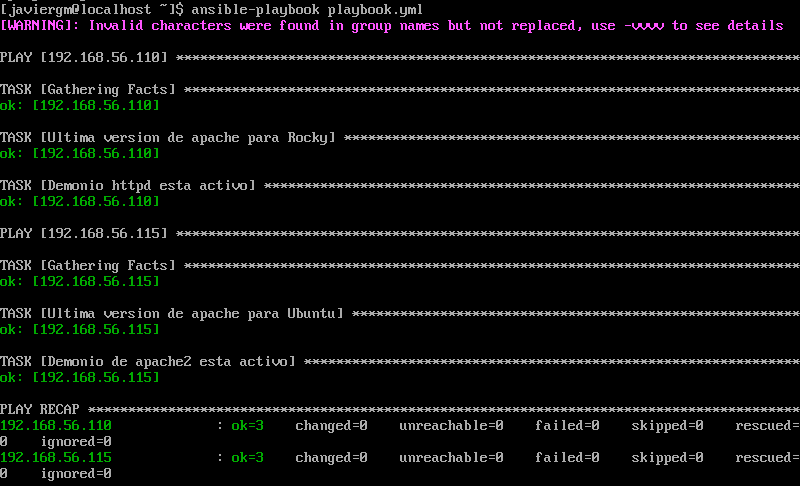
\includegraphics[scale=0.6]{Captura27}
  \caption{Playbook de Ansible}
  \label{fig:ansible-playbook-sudo}
\end{figure}

Como se puede ver en la imagen, el playbook ha funcionado a la perfección y se ha podido comprobar que los servicios de apache2 en Ubuntu y httpd en Rocky están actualizados y en funcionamiento.\\

Hay que tener en cuenta que estamos quitando formas de autenticado con la contraseña para los usuarios del grupo de wheel en Rocky y de sudo en Ubuntu, y podría ser un problema, pero si las máquinas forman parte de un grupo  de servidores que se gestionan por si solos y nadie debe de acceder a ellas, no debería haber problema con esta modificación.

\end{document}